\documentclass[12pt, twoside]{article}
\usepackage[utf8]{inputenc}
\usepackage[english]{babel}

\usepackage{graphicx, subfigure, wrapfig, float}
\usepackage{amsmath, amssymb, amsfonts, amsthm}
\usepackage{caption, multicol, multirow, longtable}
\usepackage{url, cclicenses, lastpage, color, booktabs}
\usepackage{graphicx,lipsum,wrapfig} 
\usepackage{hyperref}
\usepackage{fancyhdr, fancybox}
\usepackage{array} 
\usepackage{vmargin}
\usepackage{xcolor}



%%%%%% Begin python listling

\usepackage{xcolor}
\definecolor{maroon}{cmyk}{0, 0.87, 0.68, 0.32}
\definecolor{halfgray}{gray}{0.55}
\definecolor{ipython_frame}{RGB}{207, 207, 207}
\definecolor{ipython_bg}{RGB}{247, 247, 247}
\definecolor{ipython_red}{RGB}{186, 33, 33}
\definecolor{ipython_green}{RGB}{0, 128, 0}
\definecolor{ipython_cyan}{RGB}{64, 128, 128}
\definecolor{ipython_purple}{RGB}{170, 34, 255}

\usepackage{listings}
\lstset{
    breaklines=true,
    %
    extendedchars=true,
    literate=
    {á}{{\'a}}1 {é}{{\'e}}1 {í}{{\'i}}1 {ó}{{\'o}}1 {ú}{{\'u}}1
    {Á}{{\'A}}1 {É}{{\'E}}1 {Í}{{\'I}}1 {Ó}{{\'O}}1 {Ú}{{\'U}}1
    {à}{{\`a}}1 {è}{{\`e}}1 {ì}{{\`i}}1 {ò}{{\`o}}1 {ù}{{\`u}}1
    {À}{{\`A}}1 {È}{{\'E}}1 {Ì}{{\`I}}1 {Ò}{{\`O}}1 {Ù}{{\`U}}1
    {ä}{{\"a}}1 {ë}{{\"e}}1 {ï}{{\"i}}1 {ö}{{\"o}}1 {ü}{{\"u}}1
    {Ä}{{\"A}}1 {Ë}{{\"E}}1 {Ï}{{\"I}}1 {Ö}{{\"O}}1 {Ü}{{\"U}}1
    {â}{{\^a}}1 {ê}{{\^e}}1 {î}{{\^i}}1 {ô}{{\^o}}1 {û}{{\^u}}1
    {Â}{{\^A}}1 {Ê}{{\^E}}1 {Î}{{\^I}}1 {Ô}{{\^O}}1 {Û}{{\^U}}1
    {œ}{{\oe}}1 {Œ}{{\OE}}1 {æ}{{\ae}}1 {Æ}{{\AE}}1 {ß}{{\ss}}1
    {ç}{{\c c}}1 {Ç}{{\c C}}1 {ø}{{\o}}1 {å}{{\r a}}1 {Å}{{\r A}}1
    {€}{{\EUR}}1 {£}{{\pounds}}1,
    tabsize=2
}

%%
%% Python definition (c) 1998 Michael Weber
%% Additional definitions (2013) Alexis Dimitriadis
%% modified by me (should not have empty lines)
%%
\lstdefinelanguage{iPython}{
    morekeywords={access,and,break,class,continue,def,del,elif,else,except,exec,finally,for,from,global,if,import,in,is,lambda,not,or,pass,print,raise,return,try,while},%
    %
    % Built-ins
    morekeywords=[2]{abs,all,any,basestring,bin,bool,bytearray,callable,chr,classmethod,cmp,compile,complex,delattr,dict,dir,divmod,enumerate,eval,execfile,file,filter,float,format,frozenset,getattr,globals,hasattr,hash,help,hex,id,input,int,isinstance,issubclass,iter,len,list,locals,long,map,max,memoryview,min,next,object,oct,open,ord,pow,property,range,raw_input,reduce,reload,repr,reversed,round,set,setattr,slice,sorted,staticmethod,str,sum,super,tuple,type,unichr,unicode,vars,xrange,zip,apply,buffer,coerce,intern},%
    %
    sensitive=true,%
    morecomment=[l]\#,%
    morestring=[b]',%
    morestring=[b]",%
    %
    morestring=[s]{'''}{'''},% used for documentation text (mulitiline strings)
    morestring=[s]{"""}{"""},% added by Philipp Matthias Hahn
    %
    morestring=[s]{r'}{'},% `raw' strings
    morestring=[s]{r"}{"},%
    morestring=[s]{r'''}{'''},%
    morestring=[s]{r"""}{"""},%
    morestring=[s]{u'}{'},% unicode strings
    morestring=[s]{u"}{"}
    %
    % {replace}{replacement}{lenght of replace}
    % *{-}{-}{1} will not replace in comments and so on
    literate=
    {á}{{\'a}}1 {é}{{\'e}}1 {í}{{\'i}}1 {ó}{{\'o}}1 {ú}{{\'u}}1
    {Á}{{\'A}}1 {É}{{\'E}}1 {Í}{{\'I}}1 {Ó}{{\'O}}1 {Ú}{{\'U}}1
    {à}{{\`a}}1 {è}{{\`e}}1 {ì}{{\`i}}1 {ò}{{\`o}}1 {ù}{{\`u}}1
    {À}{{\`A}}1 {È}{{\'E}}1 {Ì}{{\`I}}1 {Ò}{{\`O}}1 {Ù}{{\`U}}1
    {ä}{{\"a}}1 {ë}{{\"e}}1 {ï}{{\"i}}1 {ö}{{\"o}}1 {ü}{{\"u}}1
    {Ä}{{\"A}}1 {Ë}{{\"E}}1 {Ï}{{\"I}}1 {Ö}{{\"O}}1 {Ü}{{\"U}}1
    {â}{{\^a}}1 {ê}{{\^e}}1 {î}{{\^i}}1 {ô}{{\^o}}1 {û}{{\^u}}1
    {Â}{{\^A}}1 {Ê}{{\^E}}1 {Î}{{\^I}}1 {Ô}{{\^O}}1 {Û}{{\^U}}1
    {œ}{{\oe}}1 {Œ}{{\OE}}1 {æ}{{\ae}}1 {Æ}{{\AE}}1 {ß}{{\ss}}1
    {ç}{{\c c}}1 {Ç}{{\c C}}1 {ø}{{\o}}1 {å}{{\r a}}1 {Å}{{\r A}}1
    {€}{{\EUR}}1 {£}{{\pounds}}1
    %
    {^}{{{\color{ipython_purple}\^{}}}}1
    {=}{{{\color{ipython_purple}=}}}1
    %
    {+}{{{\color{ipython_purple}+}}}1
    *{-}{{{\color{ipython_purple}-}}}1
    {*}{{{\color{ipython_purple}$^\ast$}}}1
    {/}{{{\color{ipython_purple}/}}}1
    %
    {+=}{{{+=}}}1
    {-=}{{{-=}}}1
    {*=}{{{$^\ast$=}}}1
    {/=}{{{/=}}}1,
    %
    identifierstyle=\color{black}\ttfamily,
    commentstyle=\color{ipython_cyan}\ttfamily,
    stringstyle=\color{ipython_red}\ttfamily,
    keepspaces=true,
    showspaces=false,
    showstringspaces=false,
    %
    rulecolor=\color{ipython_frame},
    frame=single,
    frameround={t}{t}{t}{t},
    framexleftmargin=6mm,
    xleftmargin=.28in,
    numbers=left,
    numberstyle=\tiny\color{halfgray},
    %
    %
    backgroundcolor=\color{ipython_bg},
    %   extendedchars=true,
    basicstyle=\scriptsize,
    keywordstyle=\color{ipython_green}\ttfamily,
}
%%%%%% End python listling



%%%% My usual import
\usepackage{amsmath, amsthm, amssymb, calrsfs, wasysym, verbatim, bbm, color, graphics,  enumitem, listings, tcolorbox, tikz, newtxmath, pgfplots, hyperref, paracol}

\definecolor{td}{RGB}{170,0,0}

\renewcommand\rmdefault{lmr}


%%% My commands
\newcommand\projectTitle{Computer Scientists Retrieval}
\newcommand\school{Engineering in Computer Science}


\pagestyle{fancy}
\fancyhf{}

\fancyhead[LE]{\school}
\fancyhead[RE]{\projectTitle}



\fancyhead[RO]{Academic Year 2019-2020} \fancyhead[LO]{\school}
\cfoot{\thepage}

\begin{document}
\begin{titlepage}

\setmargins{2.5cm}{1cm}{16.5cm}{23.42cm}{10pt}{1cm}{0pt}{1cm}

%encabezado portada
\begin{figure}[t]
\begin{minipage}{0.5\textwidth}\large
\begin{flushleft}
%%%%	INSERIMENTO IMMAGINE IN ALTO A SINISTRA

%
\includegraphics[scale=0.15]{ECI.png}
\end{flushleft}
\end{minipage}
\begin{minipage}{0.5\textwidth}\large
\begin{flushright}

%%%%	INSERIMENTO IMMAGINE IN ALTO A DESTRA


\includegraphics[scale=.6]{images/ECI.png}
\end{flushright}
\end{minipage}
\end{figure}

%~~~~~~~~~~~~MODIFICAR~~~~~~~~~~~~~~~~~~~~~
\title{\textsc{Computer Scientists Retrieval}} 
%~~~~~~~~~~~~~~~~~~~~~~~~~~~~~~~~~~~~~~~~~~~~
\date{}
\maketitle

\vspace{16pt}

\noindent\begin{tabular}{p{6cm} p{10cm}}
\textcolor{td}{\rule{4.5cm}{0.04cm}} 
\par\medskip
\textbf{WIR Project}
\par\bigskip
\textbf{Students:}
\begin{itemize}
%~~~~~~~~~~~~~~~~TEAM~~~~~~~~~~~~~~~~~~~~~~
\item Luca Tomei
\item Daniele Iacomini
\item Andrea Aurizi
%~~~~~~~~~~~~~~~~~~~~~~~~~~~~~~~~~~~~~~~~~~~~~~~
\end{itemize}
\par\medskip
\textbf{Directed by:}
\par\bigskip


%\par\medskip \hspace{0.5cm}
%~~~~~~~~~~~~~~~~PROFS~~~~~~~~~~~~~~~~~~~~~~
\textrm{\textit{Andrea Vitaletti}}
\par\medskip
\textrm{\textit{Luca Becchetti}}

\vspace{15pt}
\href{https://github.com/LucaTomei/Computer_Scrientists}{\underline{Project Repository}}

%~~~~~~~~~~~~~~~~~~~~~~~~~~~~~~~~~~~~~~~~~~~~~~~
\vspace{2cm} 
\par\medskip
\begin{center}
%~~~~~~~~~~~~~~~~AY~~~~~~~~~~~~~~~~~~~~~~
\textbf{A.Y. 2019-2020}
%~~~~~~~~~~~~~~~~~~~~~~~~~~~~~~~~~~~~~~~~~~~~~~~~
\end{center}
%~~~~~~~~~~~~~~~~~~~~~~~



%~~~~~~~~~~~~~~~~~~~~~~~~~~~~~~~~~~~~~~~~~~~~~~~~~~~~~~~~

\includegraphics[scale=0.4]{images/logo.png}
&

\textbf{Summary}	%Write Summary
\par\medskip
The paper we chose presents a method to find the most influential rock guitarist by applying Google’s PageRank algorithm to information extracted from Wikipedia articles. The influence of a guitarist is computed by considering the number of guitarists citing him/her as influence.
\linebreak

Basically, the experiment consists of building a directed graph where nodes are rock guitarists. There is an outgoing edge from guitarist A to another guitarist B, if guitarist A is influenced by guitarist B.
\begin{center}
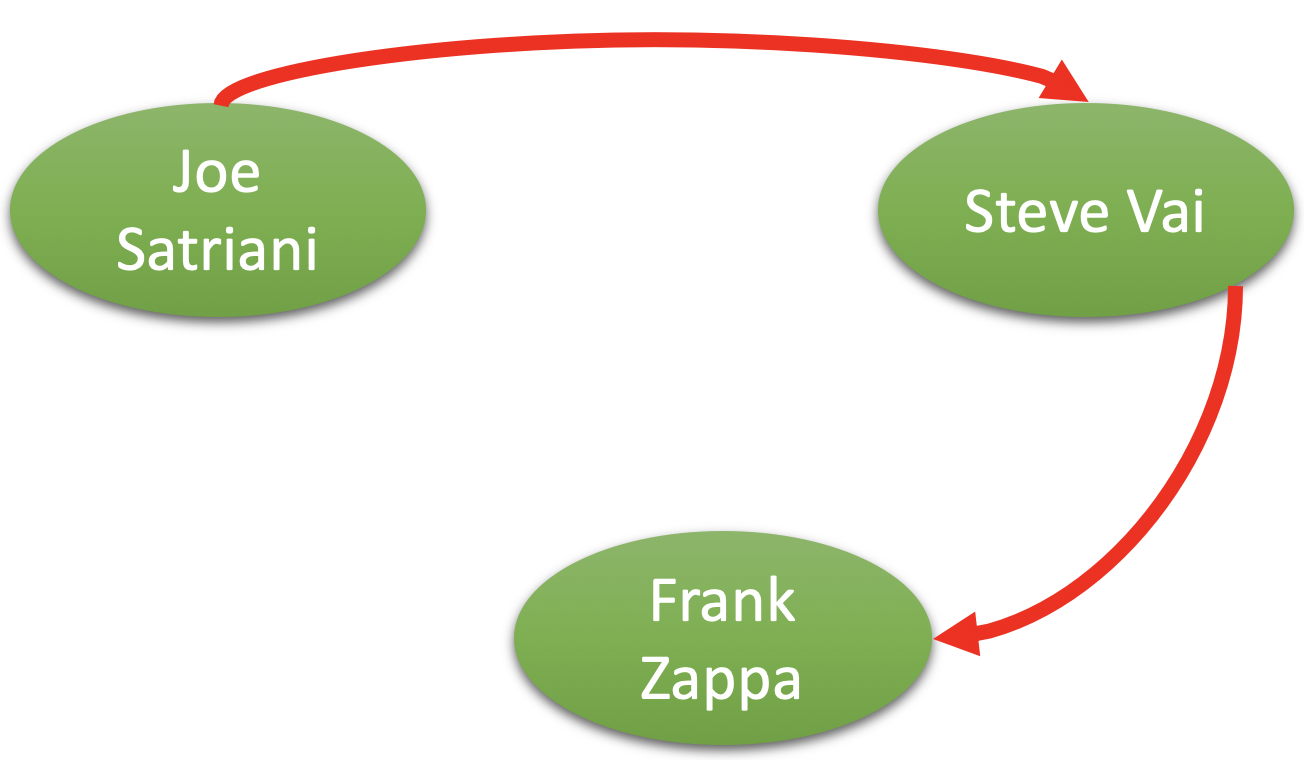
\includegraphics[scale=0.22]{images/guitar_influences}	
\linebreak
\scriptsize Joe Satriani is influenced by Steve Vai and the latter by Frank Zappa
\end{center}
We decided to replicate the same experiment with the same methodology but choosing computer scientists as the field of study.

\end{tabular}
\end{titlepage}

\tableofcontents
$\ $

\newpage
%%%%%%%%%%%%%%%%%%%%%%%%INTRODUCTION%%%%%%%%%%%%%%%%%%%%%%%%
\section{Introduction}
In questo progetto ci siamo soffermati sull'analisi dei dati riguardanti una categoria diversa da quella dei chitarristi: i computer scientists. A differenza di un chitarrista o di un filosofo, un ingegnere informatico non ha molti dati rilevanti su wikipedia e non vi sono nemmeno informazioni riguardanti la sua scuola di pensiero o le influenze avute durante la sua vita. Infatti la prima difficoltà riscontrata durante la fase preliminare del progetto è stata proprio quella di cercare di creare una corrispondenza biunivoca tra due ingegneri informatici, cosa che non sempre è possibile.

\begin{figure*}[htp]
\begin{minipage}[t]{0.5\linewidth}
\centering
	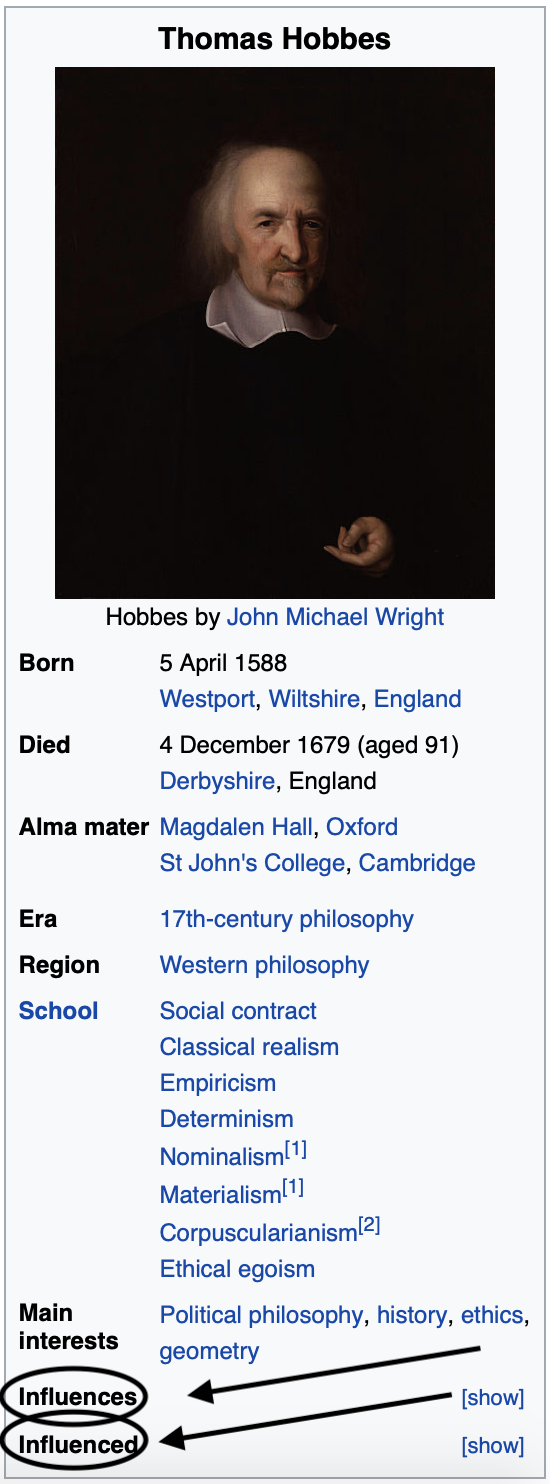
\includegraphics[width = .5\textwidth]{images/hobbes}
\end{minipage}
\begin{minipage}[t]{0.5\linewidth}
\vspace{-260pt}
\centering

\includegraphics[width = .5\textwidth]{images/van_der}
\end{minipage}
\caption{Poet vs Computer Scientist}
\end{figure*}
\noindent
Le precedenti figure mostrano i campi dati presenti sulle tabelle "infobox biography vcard" di WikiPedia. La differenza nel numero di campi tra un filosofo ed un computer scientist è netta ed inoltre quest'ultimo non presenta campi di tipo "Influences" e "Influences" a cui possiamo attingere per creare collegamenti tra un informatico ed un altro.\\
Pertanto, per ovviare a tale problema, in primo luogo si è deciso di utilizzare \textit{SPARQL} per esplorare ed estrarre le informazioni contenute in grafi RDF da una base di conoscenza distribuita su \textit{DBpedia}.\\
Successivamente si è deciso di effettuare una ulteriore verifica dei risultati andando ad interrogare direttamente Wikipedia dato che è senza dubbio una delle maggiori risorse del Web per tutte le conoscenze.

\newpage
\section{Query DBpedia with SPARQL}
Per interrogare DBpedia si è pensato di utilizzare \textit{SPARQLWrapper}, wrapper con lo scopo di a creare l'URI della query e, possibilmente, a convertire il risultato in un formato più gestibile.
\vspace{6pt}
\begin{lstlisting}[caption={Query DBpedia},captionpos=b,language=iPython]
"""Query DBpedia with SPARQL Code"""
from SPARQLWrapper import SPARQLWrapper, JSON

sparql = SPARQLWrapper("http://dbpedia.org/sparql")
sparql.setQuery("""
	PREFIX rdfs: <http://www.w3.org/2000/01/rdf-schema#>
	SELECT *
	WHERE {
		?p a
		<http://dbpedia.org/ontology/Computer_scientists> .
		?p <http://dbpedia.org/ontology/influenced> ?influenced.
	}
   """)
sparql.setReturnFormat(JSON)
results = sparql.query().convert()
\end{lstlisting}
Con i dati memorizzati in questo modo, la creazione del grafo è semplice: è sufficiente elaborare ogni riga (ognuna è costituita da due voci: influenzato e influenza) e inserire un arco corrispondente nel grafo.\\
Dopo aver incapsulato l'output della query nella variabile \lstinline[language = iPython]{result} siamo pronti ad esaminare i dati ottenuti e a creare un grafo per calcolare il pagerank.

\vspace{6pt}

\begin{lstlisting}[caption={Computing Pagerank},captionpos=b,firstnumber=35,language=iPython]
G = nx.DiGraph()

for result in results["results"]["bindings"]:
	try:
		cs = result["p"]["value"].split("/resource/")[1]
		influenced = result["influenced"]["value"].split("/resource/")[1]
		
		G.add_edge(influenced, cs)
	except:	print("",end="")

""" Computing Pagerank """
pr = nx.pagerank(G, alpha=0.85)
sorted_pr = sorted(pr.items(), key=operator.itemgetter(1))
sorted_pr.reverse()

for i in sorted_pr:	print(i)
\end{lstlisting}



\newpage

\section{Manual scraping Wikipedia}
DBpedia offre pochi risultati per i Computer Scientists, motivo per cui si è deciso di intraprendere una strada più impegnativa ma che ci restituisse più risultati: il Web Scarping.\\
Si è pensato di suddividere tale processo in 4 fasi logiche:
\begin{enumerate}[noitemsep, topsep=1pt]
	\item Collezionare in un file tutti i link di computer scientists presenti nella versione inglese di Wikipedia (\textit{\href{https://en.wikipedia.org/wiki/List_of_computer_scientists}{List Of Computer Scientists}}).
	\item Per ogni link di un informatico ottenuto dalla fase precedente, si è verificato se la relativa pagina web contenesse una tabella informazioni che includesse la lista di influenze e influenzati di tale informatico.
	\item Dai risultati ottenuti si è calcolato il Pagerank con lo scopo di quantificare l'importanza dell'informatico relativa all'interno dell'insieme di documenti connessi.
	\item Si è pensato di soffermarci sulla classificazione dei vari campi di studio di un informatico.
\end{enumerate}

\subsection{First Phase: Collect data}
The English version of Wikipedia contains a list of all the computer scientists (\textit{\href{https://en.wikipedia.org/wiki/List_of_computer_scientists}{link}}) with an existing article, alphabetically sorted. In the first phase, we simply copy each link and its associated name in a .json file.


\newpage
\section{Results}
\lipsum[1] %eliminare
\subsection{Subsection (if any)}
\lipsum %eliminare
\subsection{Subsection (if any)}
\lipsum %eliminare

\newpage
\section{Conclusions}
\lipsum[5] %eliminare
\lipsum[1] %eliminare

\newpage


\begin{thebibliography}{X} %My Bibliography
\bibitem{SPARQLWrapper}	SPARQLWrapper: \href{https://pypi.org/project/SPARQLWrapper/}{https://pypi.org/project/SPARQLWrapper/}

\bibitem{LOP} LÓPEZ, F. (SF) \textit{Espacios Topoógicos}, Depto. de Geometría y Topología, Universidad de Granada, E-18071 Granada, España
\bibitem{MACH} MACHO, M. (2002), \textit{¿Qué es la topología?}, Universidad del País Vasco-Euskal Herriko Unibertsitatea.
\bibitem{O'} O’CONNOR, J., ROBERTSON, E. (1996). \textit{A history of Topology.}
\end{thebibliography}
\end{document}



